\subsection{Case Study 2: Apache Cassandra}
\vspace{10pt}

Apache Cassandra is a Table/Key-Value hybrid NoSQL database.  It is suitable for applications that require high availability provided by replication.  In terms of the CAP theorem, Cassandra prioritizes availability and performance over consistency, making it highly performant and scalable, though consistency is eventual rather than strong, for typical Cassandra applications. % We install Apache Cassandra was on Amazon EC2 instances of various VM instance types. 
We do our testing on Cassandra clusters with 5 nodes.  
We run our testing with a replication factor of three, so every database record is stored on three of the five nodes.  We report results when using weak (or eventual) consistency, using a consistency level of ``ONE.'' We find qualitatively similar results when repeating these experiments with Cassandra's strict consistency settings that we omit due to space constraints. 

For a sample VM type that we want to predict the performance of Cassandra, we select training sets of increasing size from the remaining VM types.  We select $VM_4$ for prediction, and do multiple linear regressions on the training set for sizes 1 through 5 for read latency and write latency data.  We observe that every time another VM type is added to the training set, the associated $R^2_{predicted}$ improves for $VM_4$ for both read and write latency (see representative results in Table \ref{table:cassandra1} and Table \ref{table:cassandra2}).

These findings are also presented in an alternative way in Figure \ref{figure:cassandrabarread}, %and Figure \ref{figure:cassandrabarwrite}, 
where we plot histograms of $R^2_{predicted}$ to emphasize the improved fit associated with larger training sets of VM types.  The x-axis is labeled with sets of numbers of those VM types in each training set.

Finally, Figure \ref{figure:cassandrafitread} shows multiple linear fits offered by several training sets and shows the progressive improvement of the  model for for read latency for Cassandra as the training set grows. Figure \ref{figure:cassandrafitwrite} shows the same for write latency. We conclude that our evaluation offers supporting evidence for our second case study. 


\begin{comment}
  \begin{figure}
  \centering
    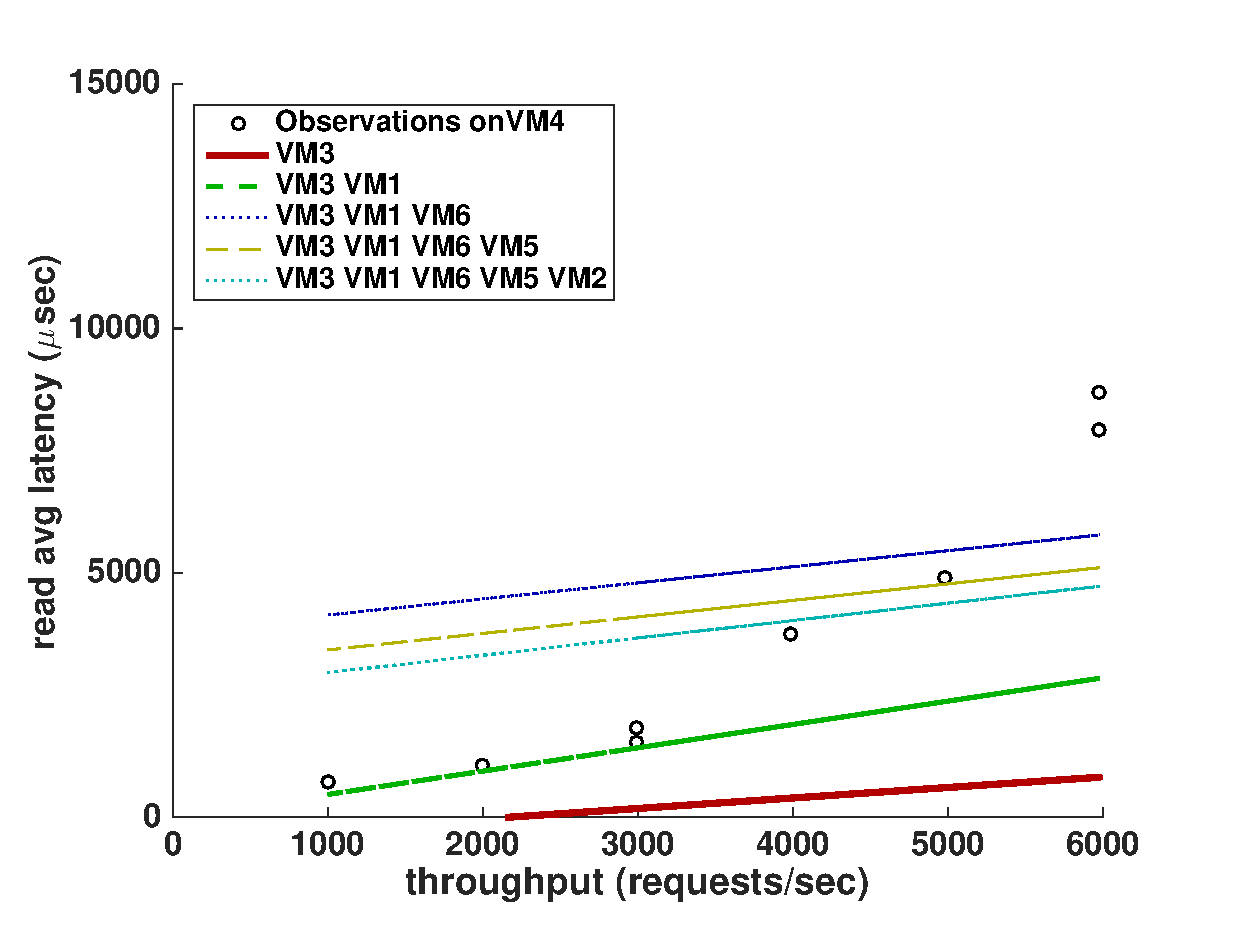
\includegraphics[scale = 0.25]{cassandra_fit_read_avg_latency_m3_2x_m3__r3_2x_r3_x_m3_x_r3_.eps}
    \caption{Cassandra average read latency vs throughput}
    \label{figure:redisbarread}
  \end{figure}

  \begin{figure}
  \centering
    \includegraphics[scale = 0.25]{cassandra_fit_read_avg_latency_r3_2x_r3_x_m3_x_m3__m3_2x_r3_.eps}
    \caption{Cassandra average read latency vs throughput}
    \label{figure:redisbarread}
  \end{figure}

  \begin{figure}
  \centering
    \includegraphics[scale = 0.25]{cassandra_fit_read_avg_latency_r3__m3_x_r3_2x_m3_2x_r3_x_m3_.eps}
    \caption{Cassandra average read latency vs throughput}
    \label{figure:redisbarread}
  \end{figure}

  \begin{figure}
  \centering
    \includegraphics[scale = 0.25]{cassandra_fit_read_avg_latency_r3_x_m3__r3_2x_m3_x_m3_2x_r3_.eps}
    \caption{Cassandra average read latency vs throughput}
    \label{figure:redisbarread}
  \end{figure}
\end{comment}

  \begin{figure}
    \centering
    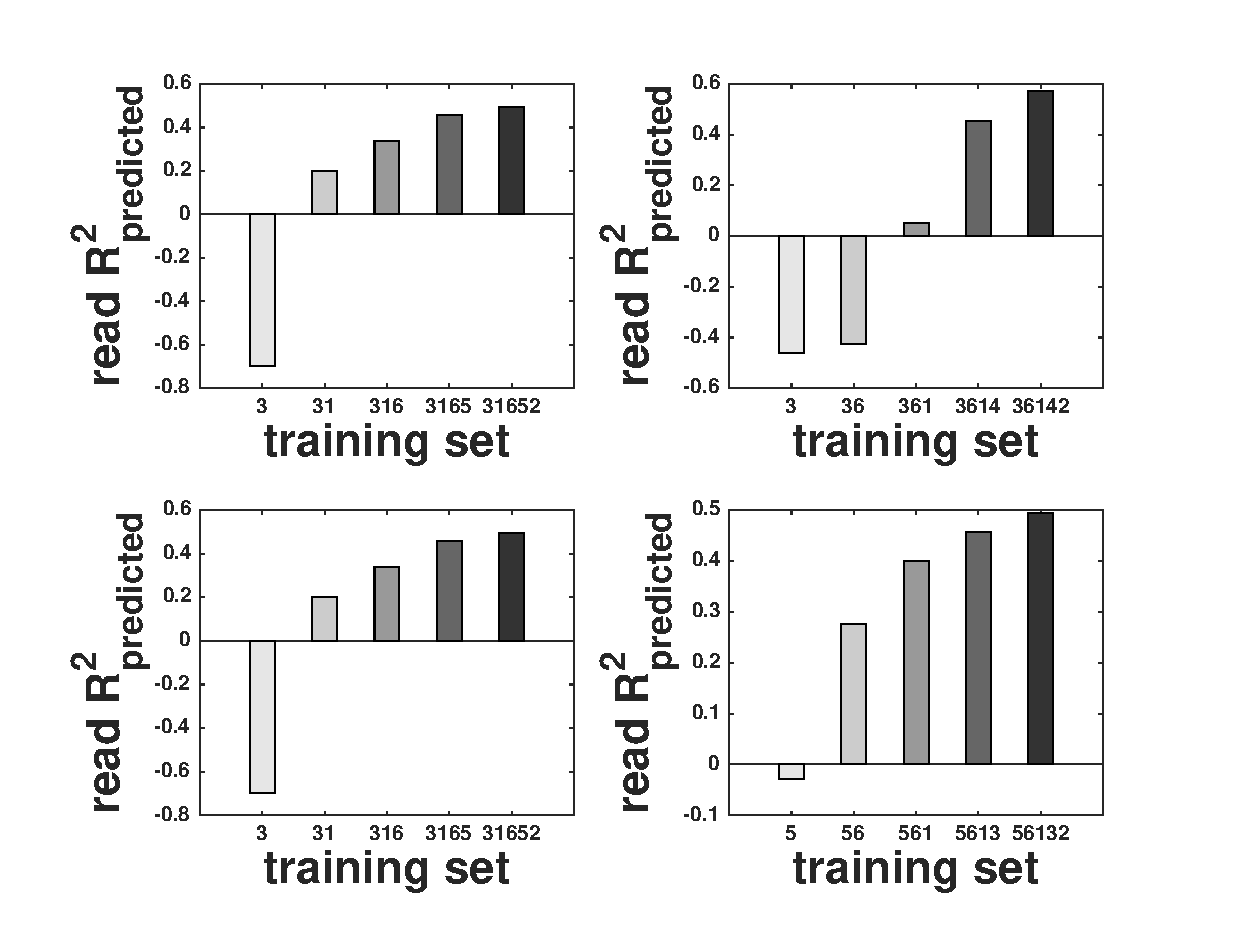
\includegraphics[scale = 0.4]{cassandra_bar_read_avg_latency.eps}
    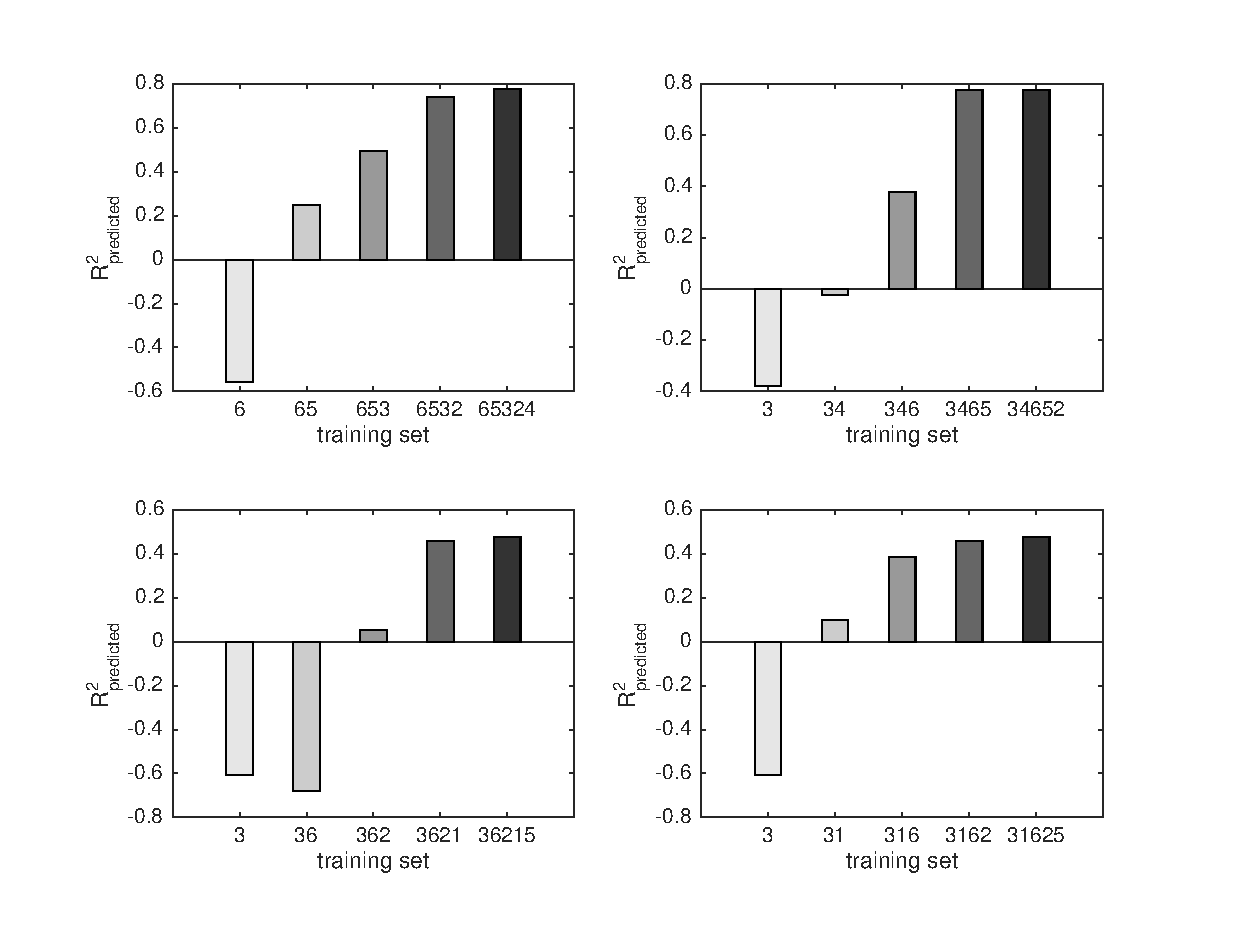
\includegraphics[scale = 0.4]{cassandra_bar_write_avg_latency.eps}
    \caption{Cassandra read and write $R^2_{predicted}$ vs training set. We find that $R^2_{predicted}$ improves consistency with more diverse training sets for a wide range of training set choices supporting our basic hypothesis.}
    \label{figure:cassandrabarread}
  \end{figure}

%   \begin{figure}
%     \centering
    
%     \caption{Cassandra write $R^2_{predicted}$ vs training set}
%     \label{figure:cassandrabarwrite}
%   \end{figure}

\begin{figure*}
\subfloat[]{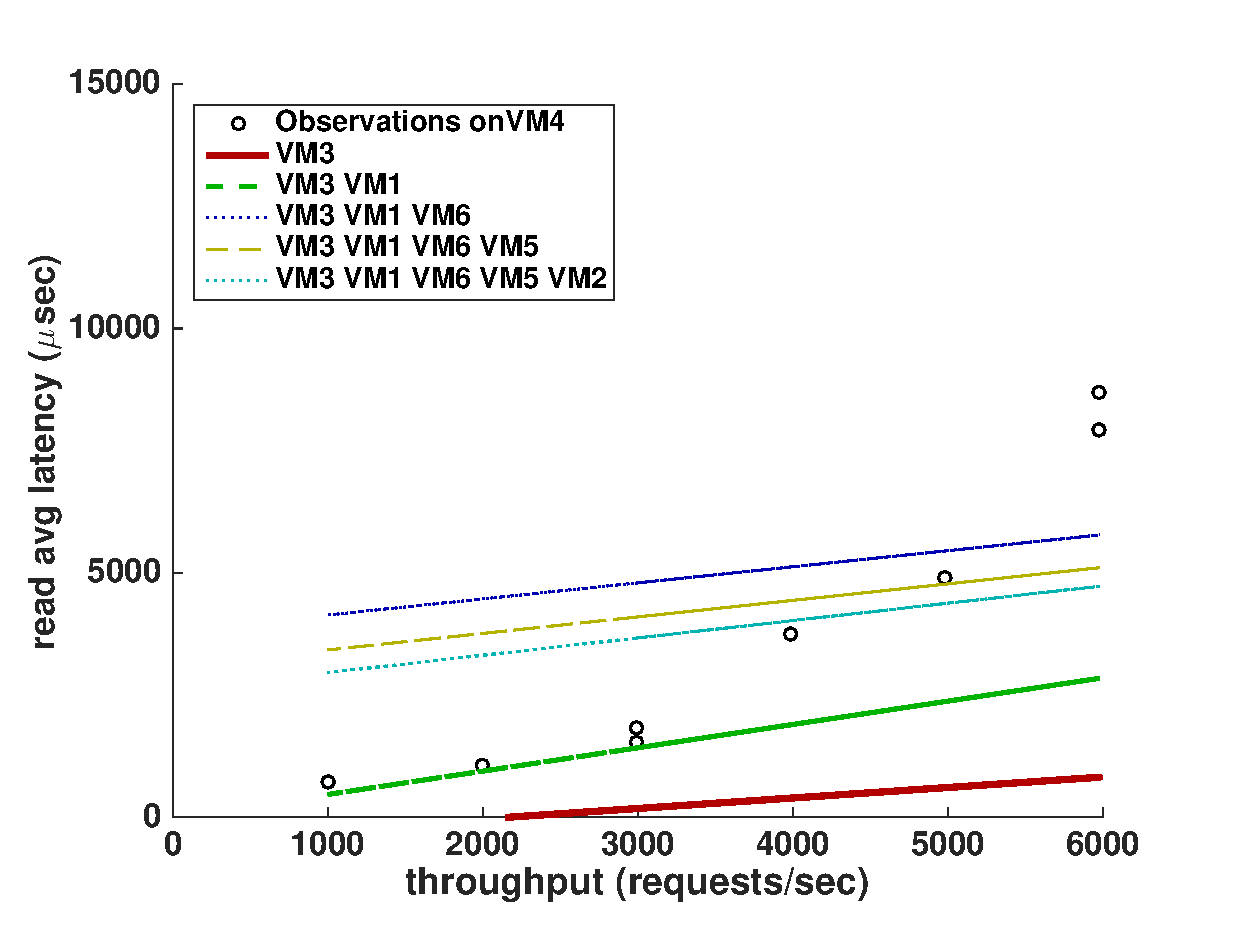
\includegraphics[width=0.25\textwidth]{cassandra_fit_read_avg_latency_m3_2x_m3__r3_2x_r3_x_m3_x_r3_.eps}} 
\subfloat[]{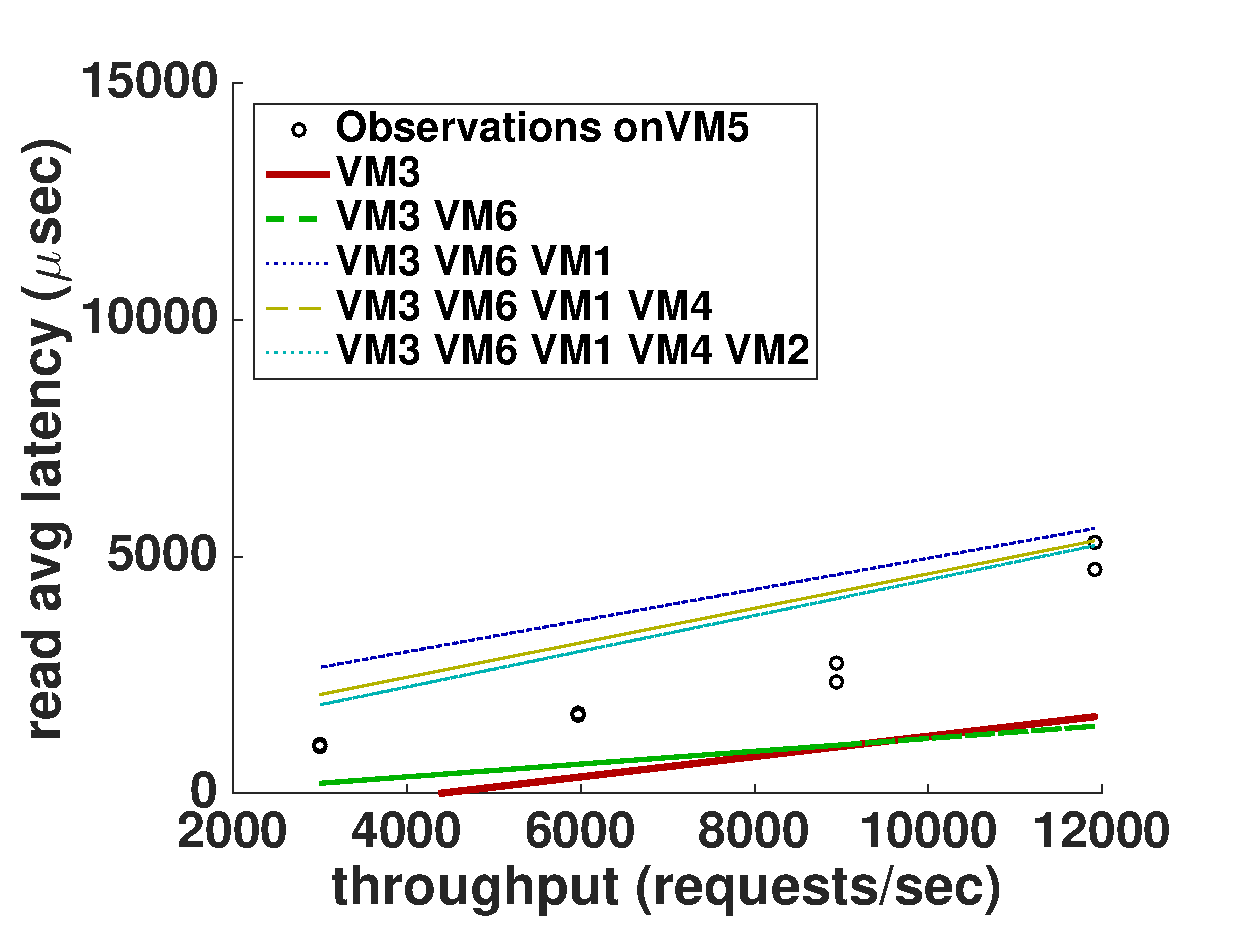
\includegraphics[width=0.25\textwidth]{cassandra_fit_read_avg_latency_m3_2x_r3_2x_m3__r3__m3_x_r3_x.eps}}
\subfloat[]{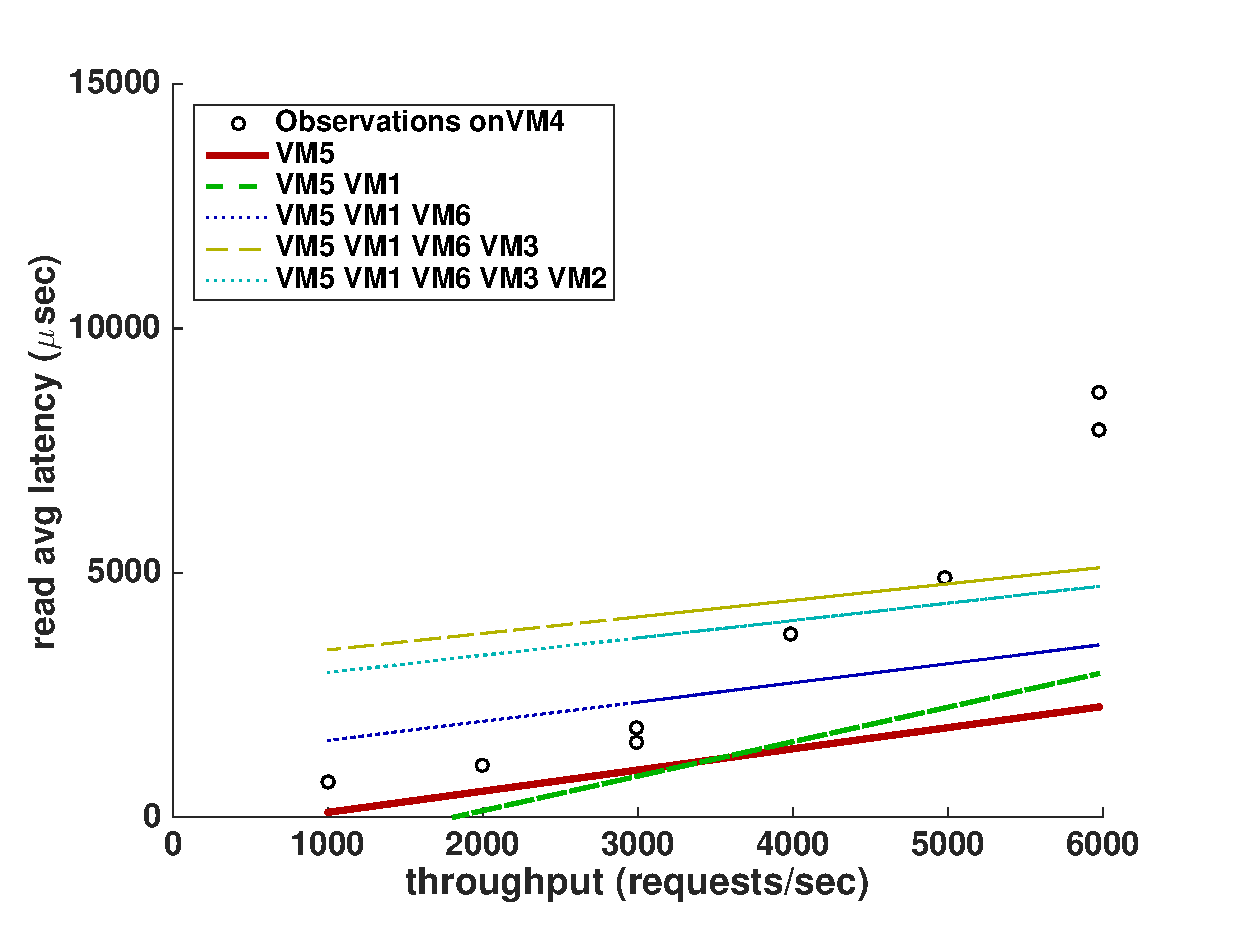
\includegraphics[width=0.25\textwidth]{cassandra_fit_read_avg_latency_r3_x_m3__r3_2x_m3_2x_m3_x_r3_.eps}}
\subfloat[]{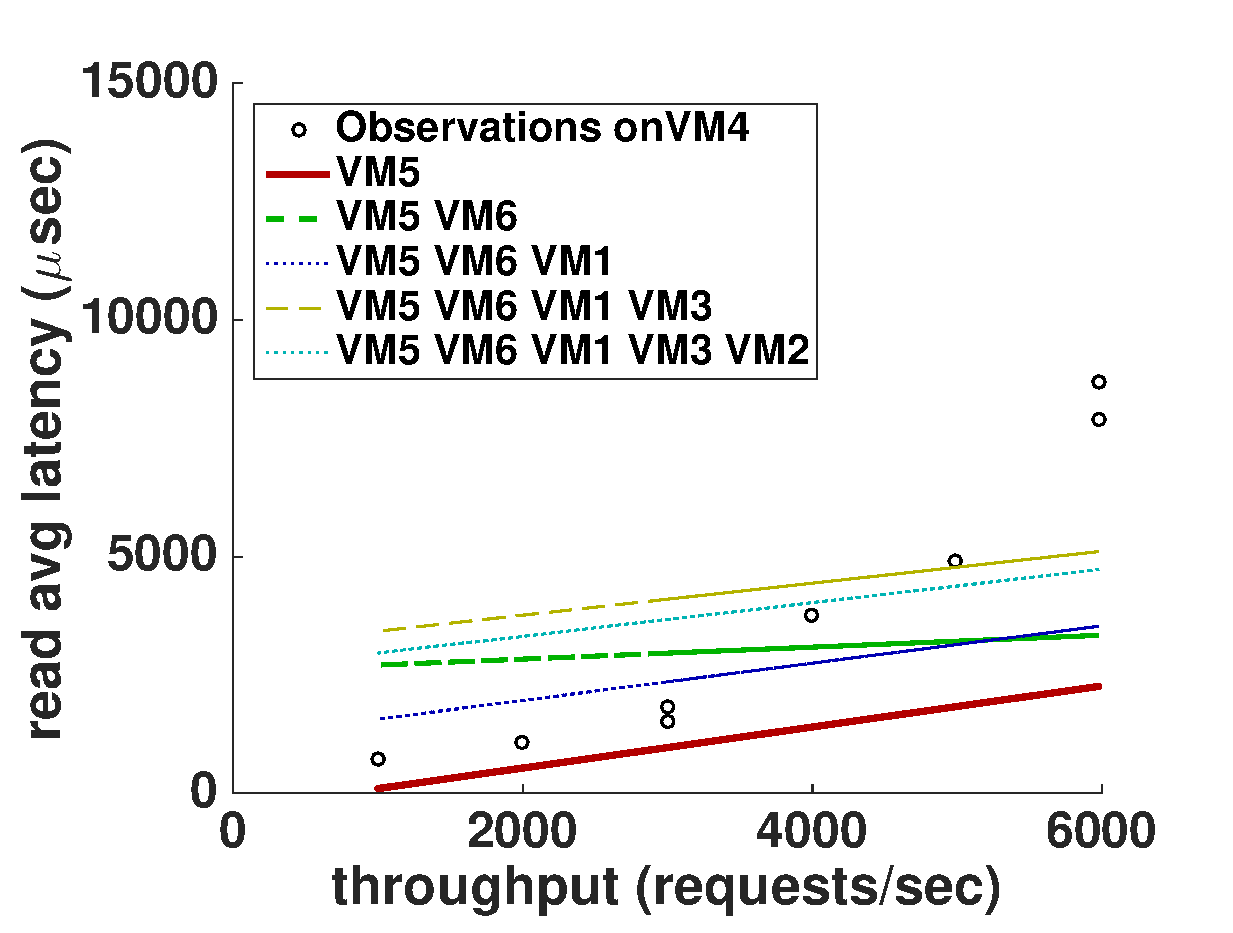
\includegraphics[width=0.25\textwidth]{cassandra_fit_read_avg_latency_r3_x_r3_2x_m3__m3_2x_m3_x_r3_.eps}}
\caption{Prediction of Cassandra read latency on $VM_4$ compared for model calibration using a variety of training sets ranging in size from 1 to 5 VM types.}
\label{figure:cassandrafitread}
\end{figure*}

\begin{comment}
  \begin{figure}
  \centering
    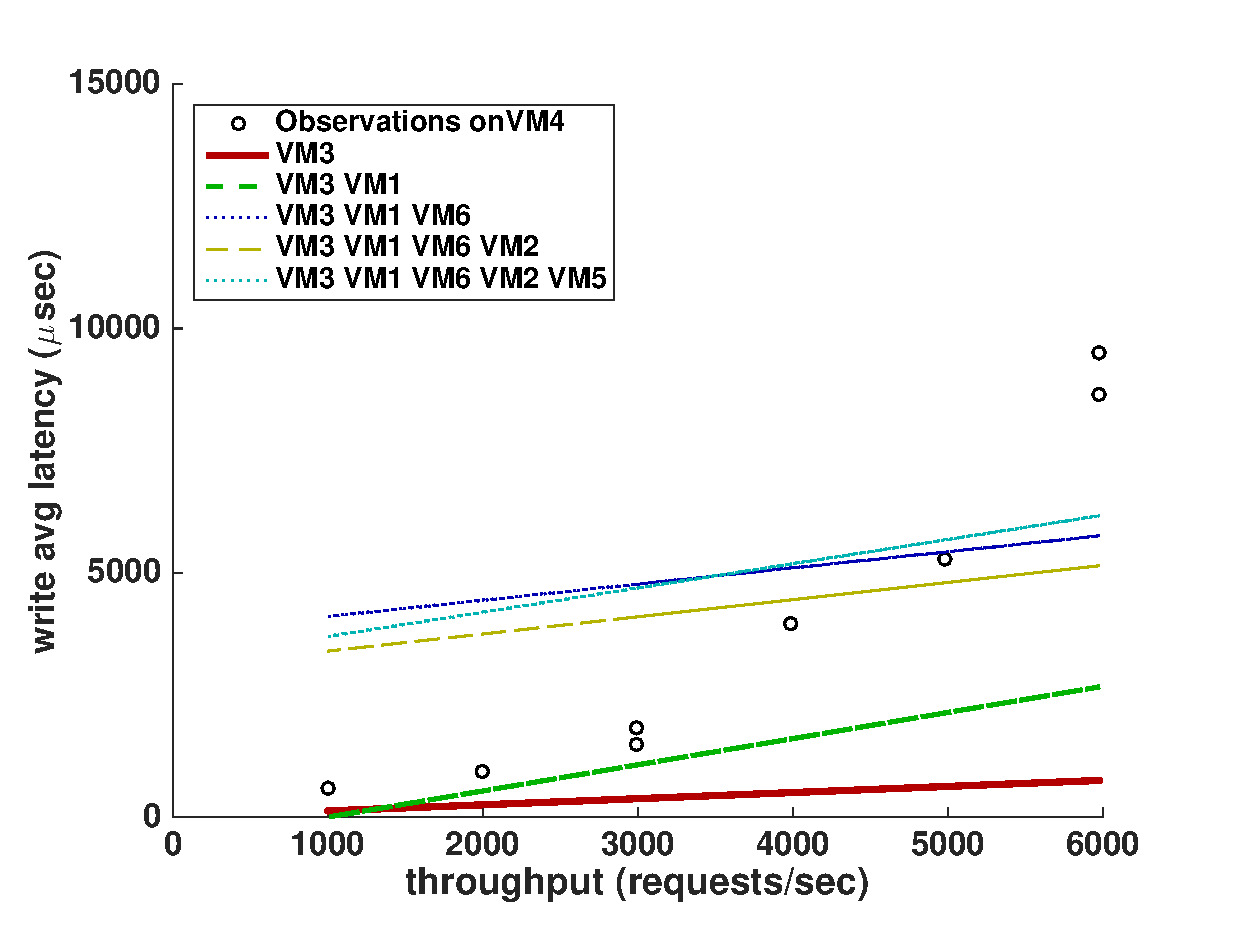
\includegraphics[scale = 0.25]{cassandra_fit_write_avg_latency_m3_2x_m3__r3_2x_m3_x_r3_x_r3_.eps}
    \caption{Cassandra average read latency vs throughput}
    \label{figure:redisbarread}
  \end{figure}

  \begin{figure}
  \centering
    \includegraphics[scale = 0.25]{cassandra_fit_write_avg_latency_m3_2x_m3_x_r3__r3_2x_r3_x_m3_.eps}
    \caption{Cassandra average read latency vs throughput}
    \label{figure:redisbarread}
  \end{figure}

  \begin{figure}
  \centering
    \includegraphics[scale = 0.25]{cassandra_fit_write_avg_latency_m3_2x_r3_x_r3_2x_m3_x_r3__m3_.eps}
    \caption{Cassandra average write latency vs throughput}
    \label{figure:redisbarread}
  \end{figure}

  \begin{figure}
  \centering
    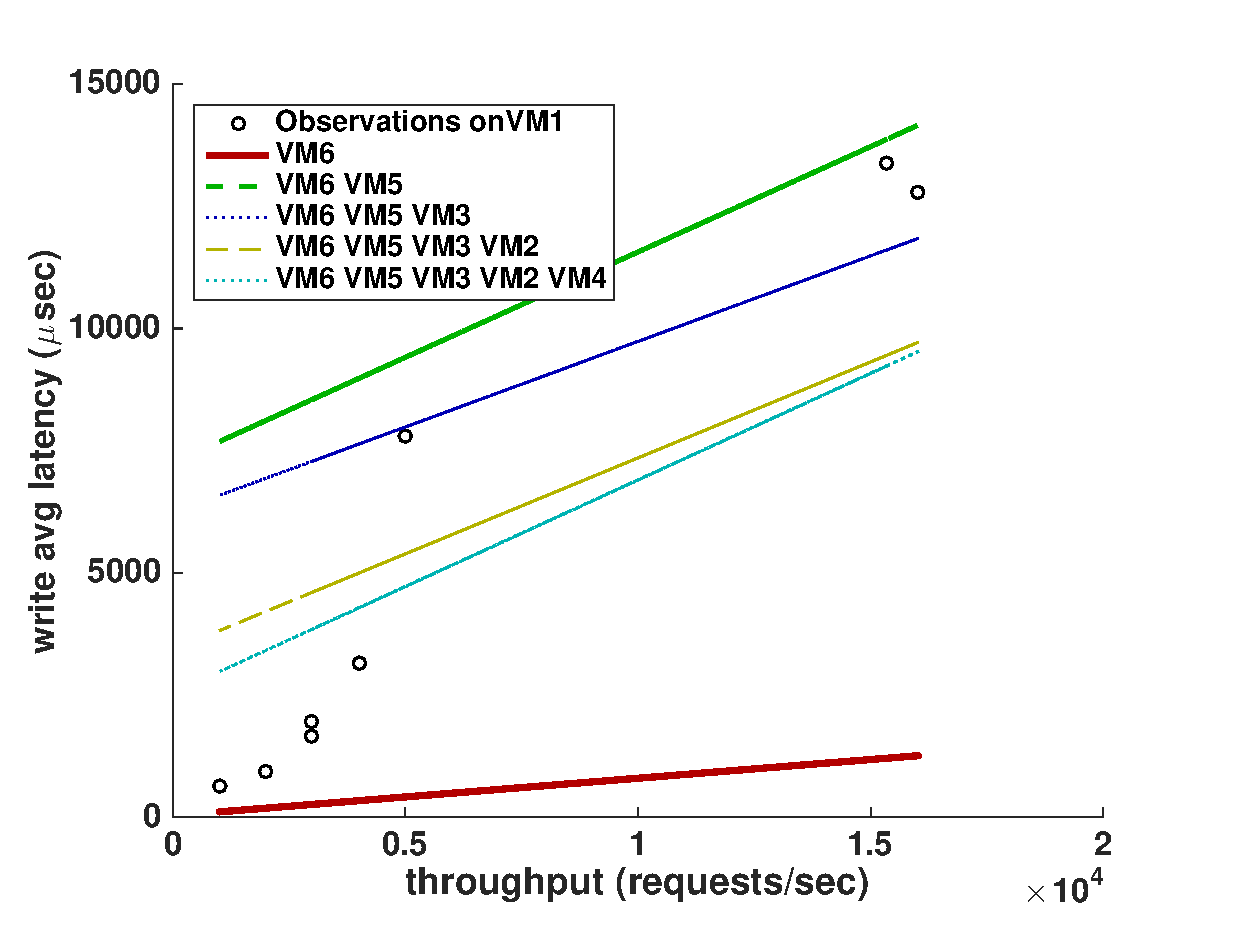
\includegraphics[scale = 0.25]{cassandra_fit_write_avg_latency_r3_2x_r3_x_m3_2x_m3_x_r3__m3_.eps}
    \caption{Cassandra average write latency vs throughput}
    \label{figure:redisbarread}
  \end{figure}
\end{comment}


\begin{figure*}
\subfloat[]{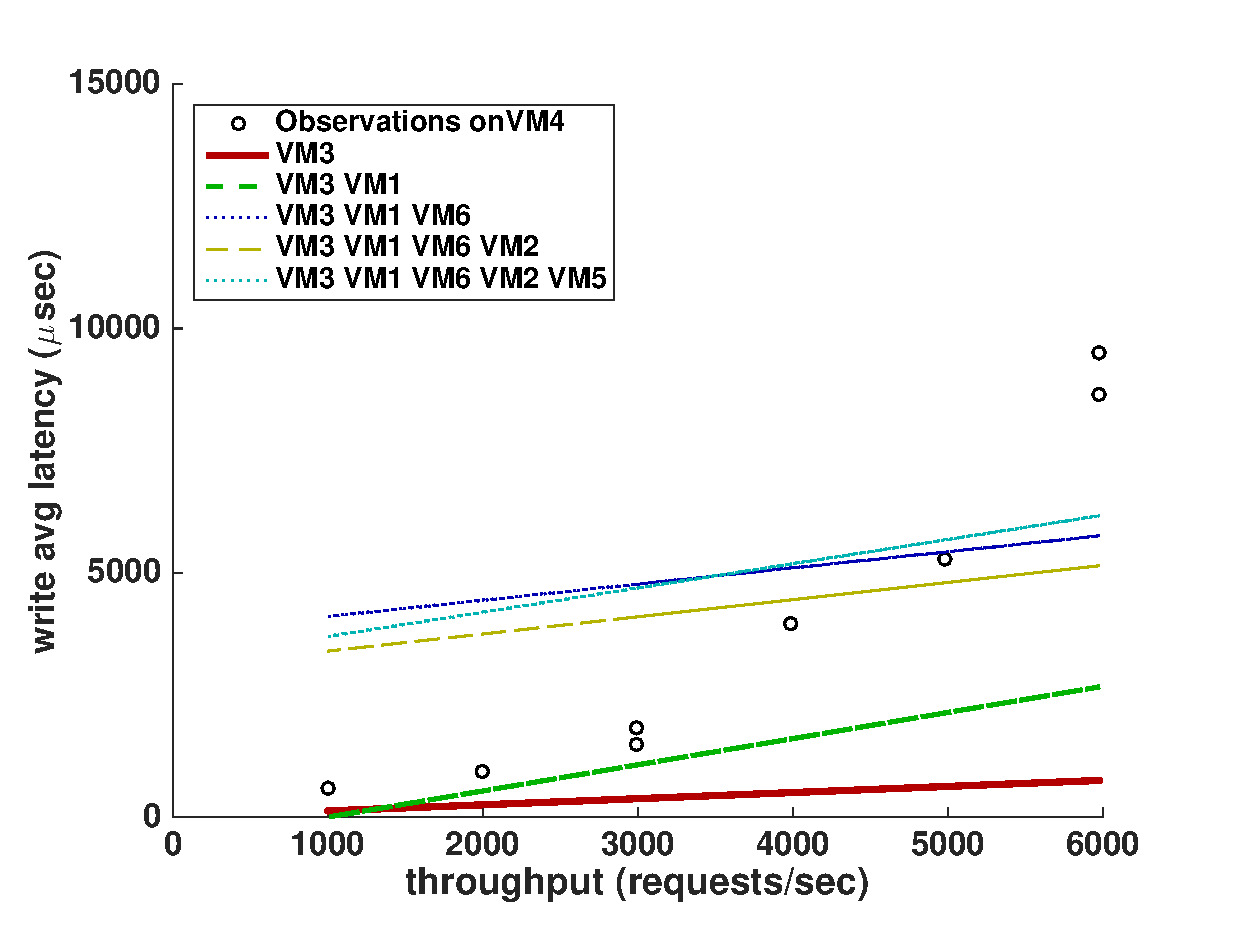
\includegraphics[width=0.25\textwidth]{cassandra_fit_write_avg_latency_m3_2x_m3__r3_2x_m3_x_r3_x_r3_.eps}} 
\subfloat[]{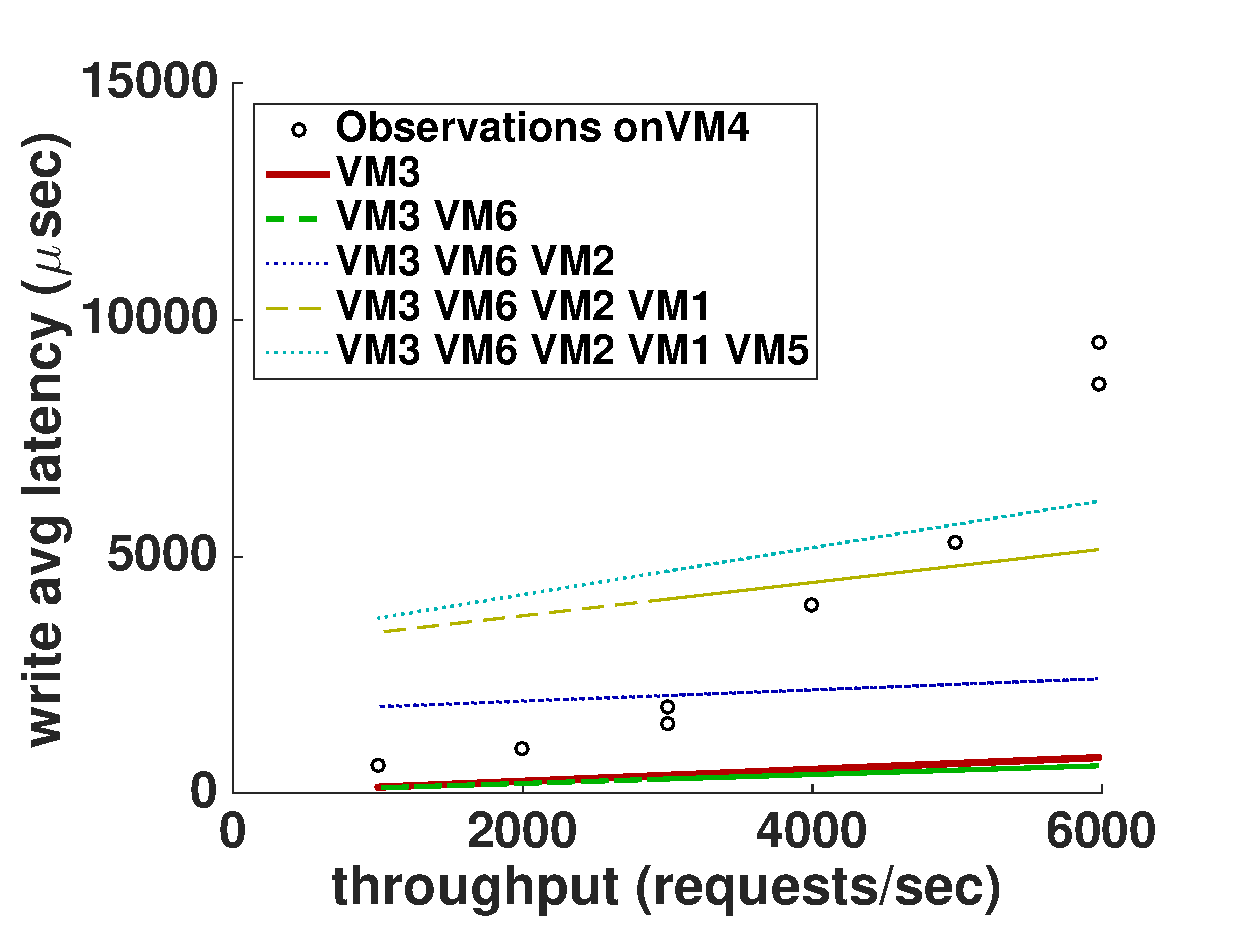
\includegraphics[width=0.25\textwidth]{cassandra_fit_write_avg_latency_m3_2x_r3_2x_m3_x_m3__r3_x_r3_.eps}}
\subfloat[]{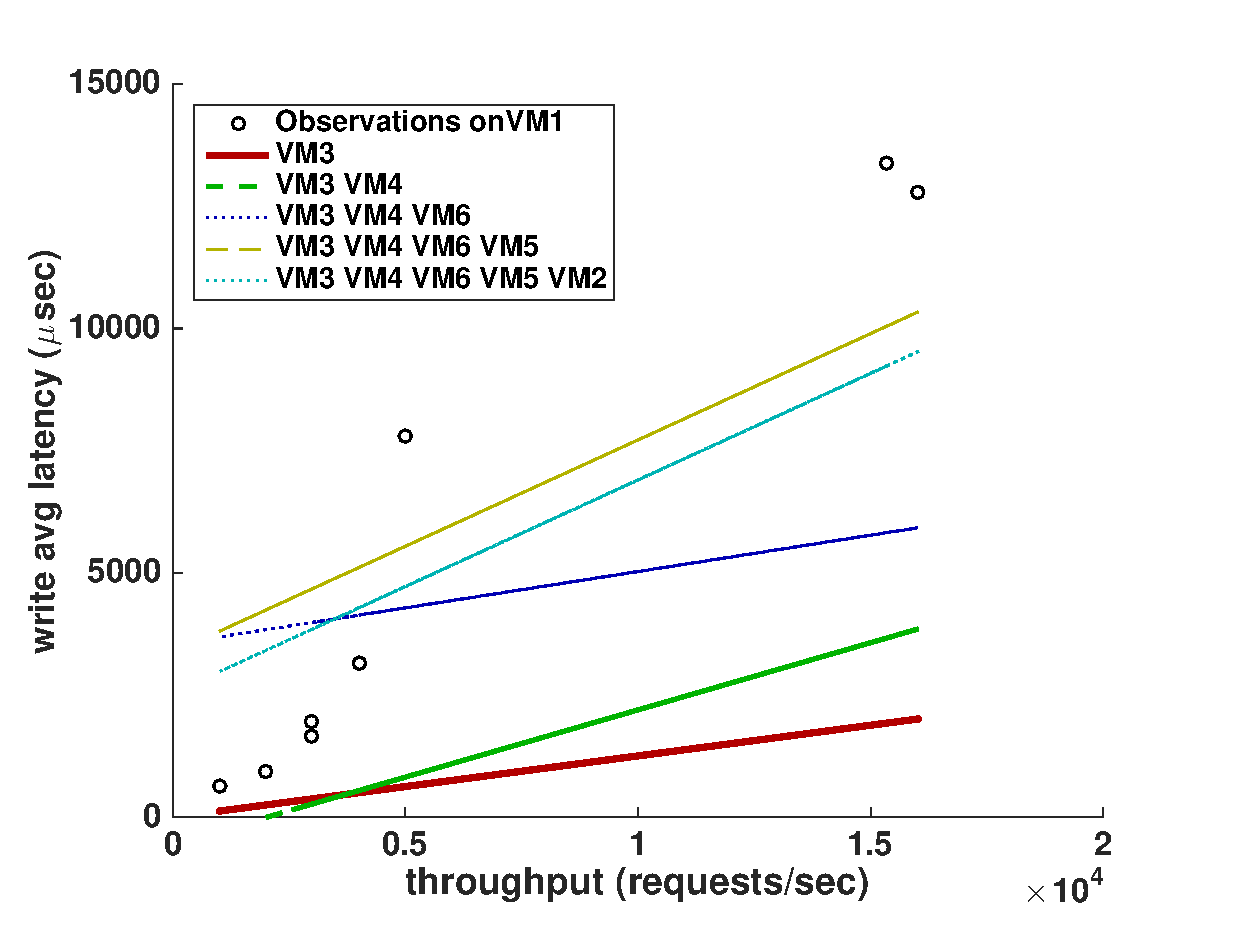
\includegraphics[width=0.25\textwidth]{cassandra_fit_write_avg_latency_m3_2x_r3__r3_2x_r3_x_m3_x_m3_.eps}}
\subfloat[]{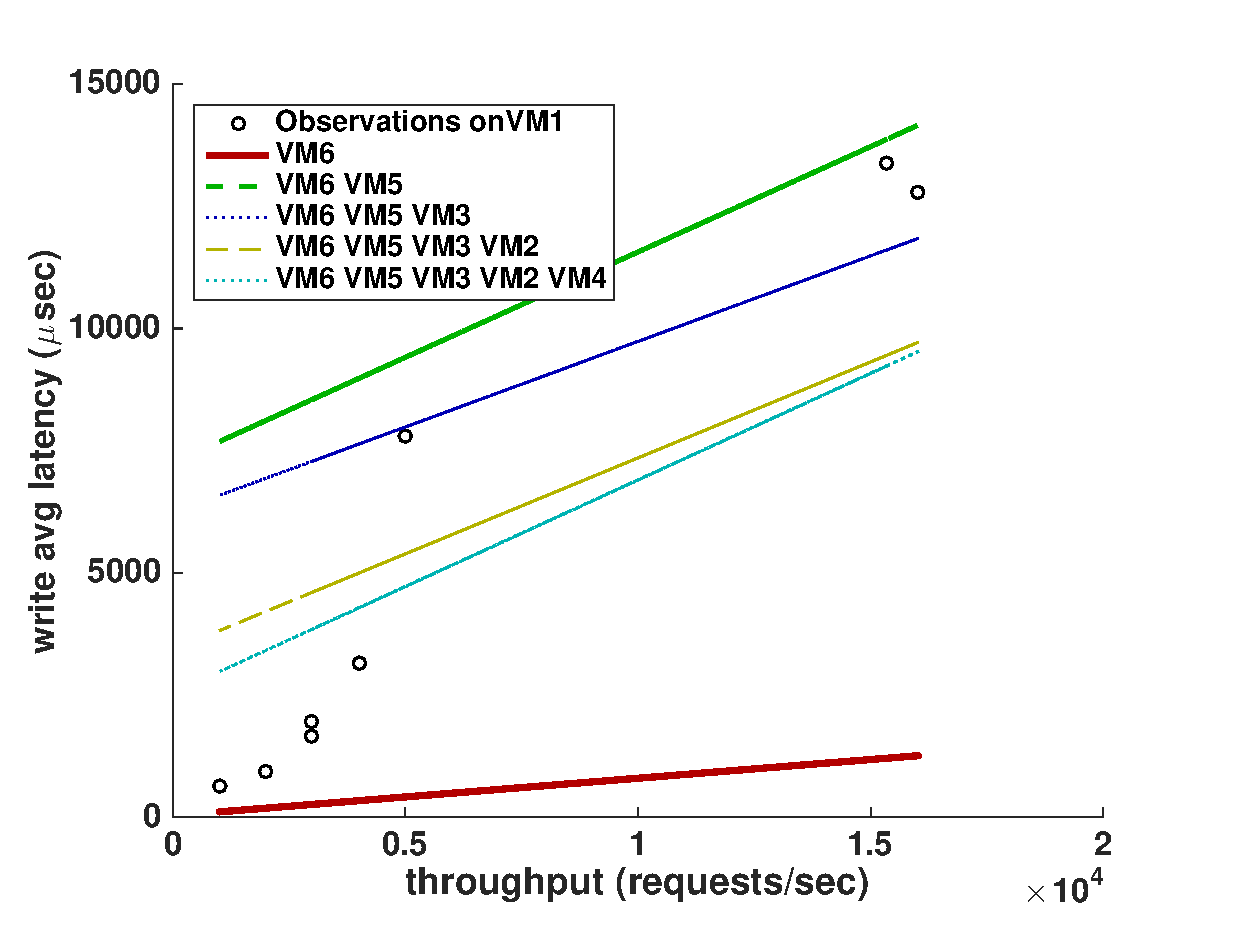
\includegraphics[width=0.25\textwidth]{cassandra_fit_write_avg_latency_r3_2x_r3_x_m3_2x_m3_x_r3__m3_.eps}} 
\caption{Prediction of Cassandra write latency on $VM_4$ compared for model calibration using a variety of training sets ranging in size from 1 to 5 VM types.}
\label{figure:cassandrafitwrite}
\end{figure*}

% \subsubsection{Evaluation for a Weak Consistency Configuration}

% consistency=ONE

% Workload B (95/5 r/w) with uniform distribution

% Present data for
% 3 VM types: gen,mem,cpu, throughputs 5000-20000, replication factor 3, 5 nodes

\begin{table}
\centering
\caption{Cassandra $R_{predicted}^2$ for $VM_4$}
\begin{tabular}{|r|r|l|} \hline
$R_{read}^2$&$R_{write}^2$&Training Data\\ \hline
-0.699345 & -0.559334  & VM3 \\ \hline 
0.199993 & 0.249826  & VM3 VM1 \\ \hline 
0.337298 &  0.495004 & VM3 VM1 VM6 \\ \hline 
0.456502 & 0.741173  & VM3 VM1 VM6 VM5 \\ \hline 
0.49455 & 0.776169  & VM3 VM1 VM6 VM5 VM2 \\ \hline 
\hline\end{tabular}
\label{table:cassandra1}
% \end{table}

% \begin{table}
\centering
\caption{Cassandra $R_{predicted}^2$ for $VM_5$}
\begin{tabular}{|r|r|l|} \hline
$R_{read}^2$&$R_{write}^2$&Training Data\\ \hline
-0.462405 & -0.380705  & VM3 \\ \hline 
-0.425988 &  -0.0225972 & VM3 VM6 \\ \hline 
0.053444 &  0.379236 & VM3 VM6 VM1 \\ \hline 
0.453755 & 0.775494  & VM3 VM6 VM1 VM4 \\ \hline 
0.574078 & 0.776169  & VM3 VM6 VM1 VM4 VM2 \\ \hline 
\hline\end{tabular}
\label{table:cassandra2}
% \end{table}

% \begin{table}
\centering
\caption{Cassandra $R_{predicted}^2$ for $VM_4$}
\begin{tabular}{|r|r|l|} \hline
$R_{read}^2$&$R_{write}^2$&Training Data\\ \hline
-0.0293728 & -0.605137  & VM5 \\ \hline 
0.157659 &  -0.681656 & VM5 VM1 \\ \hline 
0.400541 & 0.0545588  & VM5 VM1 VM6 \\ \hline 
0.456502 & 0.459396  & VM5 VM1 VM6 VM3 \\ \hline 
0.49455 & 0.477652  & VM5 VM1 VM6 VM3 VM2 \\ \hline 
\hline\end{tabular}
\label{table:cassandra3}
% \end{table}

% \begin{table}
\centering
\caption{Cassandra $R_{predicted}^2$ for $VM_4$}
\begin{tabular}{|r|r|l|} \hline
$R_{read}^2$&$R_{write}^2$&Training Data\\ \hline
-0.0293728 & -0.605137  & VM5 \\ \hline 
0.276549 & 0.0974061  & VM5 VM6 \\ \hline 
0.400541 & 0.385513  & VM5 VM6 VM1 \\ \hline 
0.456502 &  0.459396 & VM5 VM6 VM1 VM3 \\ \hline 
0.49455 &  0.477652 & VM5 VM6 VM1 VM3 VM2 \\ \hline 
\hline\end{tabular}
\label{table:cassandra4}
\end{table}
